% Created 2022-10-19 on 17:03
% Intended LaTeX compiler: pdflatex
\documentclass[table]{beamer}

%%%% settings when exporting code %%%% 

\usepackage{listings}
\lstdefinestyle{code-small}{
backgroundcolor=\color{white}, % background color for the code block
basicstyle=\ttfamily\small, % font used to display the code
commentstyle=\color[rgb]{0.5,0,0.5}, % color used to display comments in the code
keywordstyle=\color{black}, % color used to highlight certain words in the code
numberstyle=\ttfamily\tiny\color{gray}, % color used to display the line numbers
rulecolor=\color{black}, % color of the frame
stringstyle=\color[rgb]{0,.5,0},  % color used to display strings in the code
breakatwhitespace=false, % sets if automatic breaks should only happen at whitespace
breaklines=true, % sets automatic line breaking
columns=fullflexible,
frame=single, % adds a frame around the code (non,leftline,topline,bottomline,lines,single,shadowbox)
keepspaces=true, % % keeps spaces in text, useful for keeping indentation of code
literate={~}{$\sim$}{1}, % symbol properly display via latex
numbers=none, % where to put the line-numbers; possible values are (none, left, right)
numbersep=10pt, % how far the line-numbers are from the code
showspaces=false,
showstringspaces=false,
stepnumber=1, % the step between two line-numbers. If it's 1, each line will be numbered
tabsize=1,
xleftmargin=0cm,
emph={anova,apply,class,coef,colnames,colNames,colSums,dim,dcast,for,ggplot,head,if,ifelse,is.na,lapply,list.files,library,logLik,melt,plot,require,rowSums,sapply,setcolorder,setkey,str,summary,tapply},
aboveskip = \medskipamount, % define the space above displayed listings.
belowskip = \medskipamount, % define the space above displayed listings.
lineskip = 0pt} % specifies additional space between lines in listings
\lstset{style=code-small}
%%%% packages %%%%%

\usepackage[utf8]{inputenc}
\usepackage[T1]{fontenc}
\usepackage{lmodern}
\usepackage{textcomp}
\usepackage{color}
\usepackage{graphicx}
\usepackage{grffile}
\usepackage{wrapfig}
\usepackage{rotating}
\usepackage{longtable}
\usepackage{multirow}
\usepackage{multicol}
\usepackage{changes}
\usepackage{pdflscape}
\usepackage{geometry}
\usepackage[normalem]{ulem}
\usepackage{amssymb}
\usepackage{amsmath}
\usepackage{amsfonts}
\usepackage{dsfont}
\usepackage{array}
\usepackage{ifthen}
\usepackage{hyperref}
\usepackage{natbib}
\subtitle{}
\setbeamertemplate{footline}[frame number]
\setbeamertemplate{navigation symbols}{}
%
%%%% specifications %%%%
%
\usepackage{ifthen}
\usepackage{xifthen}
\usepackage{xargs}
\usepackage{xspace}
\newcommand\Rlogo{\textbf{\textsf{R}}\xspace} %
\RequirePackage{fancyvrb}
\DefineVerbatimEnvironment{verbatim}{Verbatim}{fontsize=\small,formatcom = {\color[rgb]{0.5,0,0}}}
\RequirePackage{enumitem}
\RequirePackage{changepage} % widen margin
\RequirePackage{colortbl} % arrayrulecolor to mix colors
\RequirePackage{pifont}
\RequirePackage{relsize}
\newcommand{\Cross}{{\raisebox{-0.5ex}%
{\relsize{1.5}\ding{56}}}\hspace{1pt} }
\newcommand{\Valid}{{\raisebox{-0.5ex}%
{\relsize{1.5}\ding{52}}}\hspace{1pt} }
\newcommand{\CrossR}{ \textcolor{red}{\Cross} }
\newcommand{\ValidV}{ \textcolor{green}{\Valid} }
\usepackage{stackengine}
\usepackage{scalerel}
\newcommand\Warning[1][3ex]{%
\renewcommand\stacktype{L}%
\scaleto{\stackon[1.3pt]{\color{red}$\triangle$}{\tiny\bfseries !}}{#1}%
\xspace
}
\usepackage{changepage}
\usepackage{booktabs}
\newcommand{\darkgreen}{green!50!black}
\definecolor{purplebox1}{rgb}{0.84, 0.84, 0.9375}
\definecolor{purplebox2}{rgb}{0.96, 0.96, 0.91}
\newenvironment{blueblock}[1]{%
\setbeamercolor{block title}{bg=purplebox1,fg=title.fg}
\setbeamercolor{block body}{bg=purplebox2,fg=normal text.fg}
\begin{block}{#1}}{\end{block}}
\RequirePackage{epstopdf} % to be able to convert .eps to .pdf image files
\RequirePackage{capt-of} %
\RequirePackage{caption} % newlines in graphics
\newcommand{\backupbegin}{
\newcounter{finalframe}
\setcounter{finalframe}{\value{framenumber}}
}
\newcommand{\backupend}{
\setcounter{framenumber}{\value{finalframe}}
}
\RequirePackage{hanging}
\setbeamertemplate{footnote}{%
\hangpara{2em}{1}%
\makebox[2em][l]{\insertfootnotemark}\footnotesize\insertfootnotetext\par%
}
\usetheme[height=20pt]{Singapore}
\author{Brice Ozenne}
\date{\today}
\title{"How to" in orgmode}
\hypersetup{
 colorlinks=true,
 pdfauthor={Brice Ozenne},
 pdftitle={"How to" in orgmode},
 pdfkeywords={},
 pdfsubject={},
 pdfcreator={Emacs 27.2 (Org mode 9.5.2)},
 pdflang={English}
 }
\begin{document}

\maketitle

\section{Box}
\label{sec:org6e4b5ce}

\begin{frame}[label={sec:orgd59bb64}]{Default box}
\begin{block}{Nested models}
	Consider two models $ \mathcal{M}_0 $ and $ \mathcal{M} $
\end{block}
\end{frame}

\begin{frame}[label={sec:org5616252}]{Round box}
\setbeamercolor{block title example}{fg=black,bg=lightgray}
\setbeamercolor{block body example}{fg=white,bg=gray}
\setbeamercolor{block body}{fg=white,bg=blue!60}

\begin{block}{}
	The \texttt{beamercolorbox} environment!
\end{block}

\begin{exampleblock}{block title}
	Box type \texttt{beamerboxesrounded}
	
	with shadow.
	
	Different colours are possible for the header and box contents. \ldots
\end{exampleblock}

\setbeamertemplate{blocks}[rounded][shadow=true]
\begin{example}
	Box type \texttt{beamerboxesrounded}
	
	with shadow.
	
	Different colours are possible for the header and box contents. \ldots
\end{example}
\end{frame}

\section{Code}
\label{sec:org6bb3e72}

\begin{frame}[label={sec:org51fffe3},fragile]{Set output size}
 \lstset{language=r,label= ,caption= ,captionpos=b,numbers=none}
\begin{lstlisting}
summary(model)
\end{lstlisting}


{
\RecustomVerbatimEnvironment{verbatim}{Verbatim}{fontsize=\scriptsize,formatcom = {\color[rgb]{0.5,0,0}}}

\begin{verbatim}
________________________________________________________________________________
Layer (type)                        Output Shape                    Param #     
================================================================================
dense_22 (Dense)                    (None, 256)                     200960      
________________________________________________________________________________
dense_23 (Dense)                    (None, 128)                     32896       
________________________________________________________________________________
dense_24 (Dense)                    (None, 10)                      1290        
================================================================================
Total params: 235,146
Trainable params: 235,146
Non-trainable params: 0
________________________________________________________________________________
\end{verbatim}

}

\lstset{language=r,label= ,caption= ,captionpos=b,numbers=none}
\begin{lstlisting}
model$weights[[1]]
\end{lstlisting}

{
\RecustomVerbatimEnvironment{verbatim}{Verbatim}{fontsize=\scriptsize,formatcom = {\color[rgb]{0.5,0,0}}}

\begin{verbatim}
<tf.Variable 'dense_4/kernel:0' shape=(784, 256) dtype=float32_ref>
\end{verbatim}


}
\end{frame}
\begin{frame}[label={sec:org86d8756},fragile]{Inline R}
 Bla \texttt{2}.
\end{frame}

\section{List}
\label{sec:orgeecd729}

\begin{frame}[label={sec:org08287cb}]{Choose item}
\begin{description}
\item[{(A)}] yyy
\item[{(1)}] xxx
\end{description}
\end{frame}

\begin{frame}[label={sec:orgeb4841f}]{Use itemize and modify vertical space}
\begin{itemize}[label={-},topsep=0pt,itemsep=0mm]
\item a
\item b
\item c
\end{itemize}
\end{frame}

\begin{frame}[label={sec:org9d5a6e7}]{change color}
\end{frame}

\begin{frame}[label={sec:orgb9739f0}]{label scheme}
\begin{itemize}
\item level 1: \textbullet
\item level 2: \textendash
\item level 3: \textasteriskcentered
\item level 4: \textperiodcentered
\end{itemize}
\end{frame}

\section{Table}
\label{sec:org2d37994}

\begin{frame}[label={sec:orgad9f8de}]{Nice latex table}
(require booktabs)

\begin{table}
\begin{tabular}{lll}
\toprule
A  & \textcolor{orange}{B} & \textcolor{blue}{C} \\
D & (n=282)  & (n=280) \\
\midrule
Grade 1 & 48 (17\%)  & 69 (24.6\%) \\
Grade 2 & 118 (41.8\%)  & 89 (31.5\%) \\
Grade 3 & 72 (25.5\%)  & 47 (16.8\%) \\
Grade 4 & 11 (3.9\%) & 6 (2.1\%) \\
Grade 5 & 4 (1.4\%)  & 3 (1.1\%) \\
\bottomrule
\end{tabular}
\end{table}
\end{frame}

\section{References}
\label{sec:orge5ade68}

\begin{frame}[label={sec:orge108de5}]{Citations}
\begin{itemize}
\item \citep{pearson1905problem}
\item \cite{pearson1905problem}
\item \citep[xx]{pearson1905problem}
\end{itemize}
\cite[p.~150]{pearson1905problem}
\end{frame}

\section{Miscellaneous}
\label{sec:org0479b17}

\begin{frame}[label={sec:org9b88869}]{Divide the page (align at the middle)}
\begin{columns}
\begin{column}{0.45\columnwidth}
\begin{itemize}
\item topic
\begin{itemize}
\item subtopic
\item sub
\end{itemize}
\item topic
\end{itemize}
\end{column}

\begin{column}{0.45\columnwidth}
\begin{center}
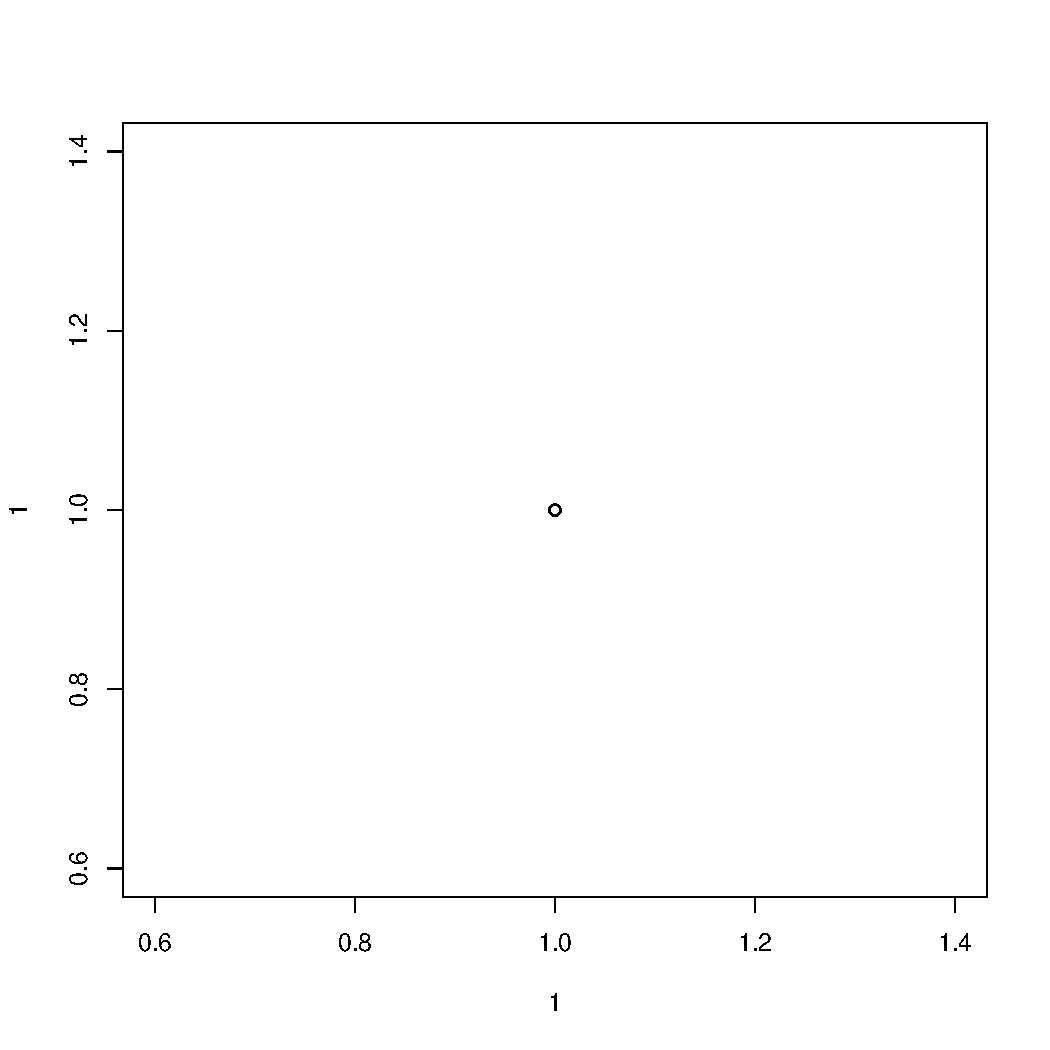
\includegraphics[width=.9\linewidth]{./figures/myplot.pdf}
\end{center}
\end{column}
\end{columns}
\end{frame}

\begin{frame}[label={sec:org57ca2a0}]{Divide the page (align at the top)}
\begin{columns}
\begin{column}[t]{0.45\columnwidth}
\begin{itemize}
\item topic
\begin{itemize}
\item subtopic
\item sub
\end{itemize}
\item topic
\end{itemize}
\end{column}

\begin{column}[T]{0.45\columnwidth}
\begin{center}
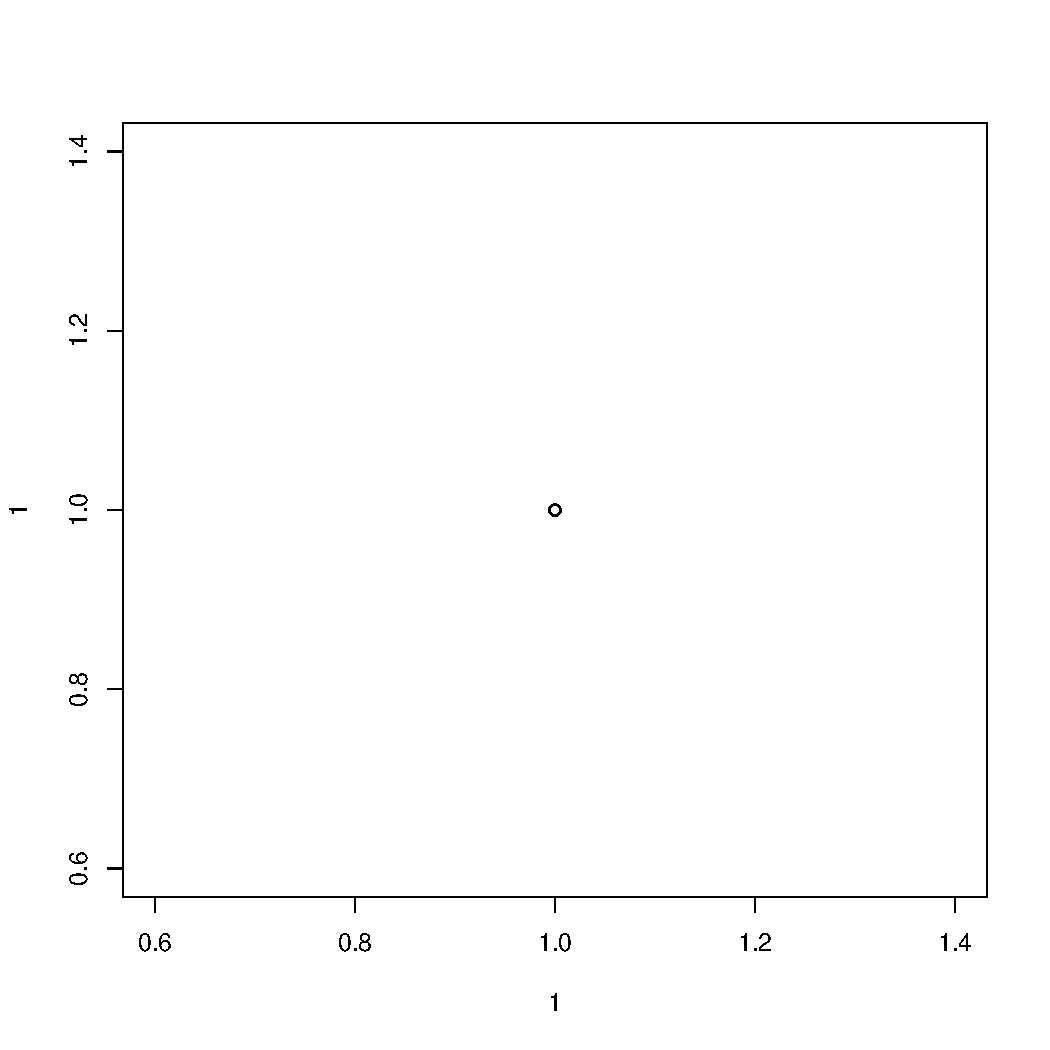
\includegraphics[width=.9\linewidth]{./figures/myplot.pdf}
\end{center}
\end{column}
\end{columns}
\end{frame}

\begin{frame}[label={sec:org2f691a1}]{Inline latex}
any arbitrary LaTeX code
\end{frame}

\begin{frame}[label={sec:org994b196}]{Color tex}
(see header for the definition of darkgreen)
\begin{itemize}
\item \textcolor{\darkgreen}{risk factor}: adjust (will increase precision)
\end{itemize}
\end{frame}

\begin{frame}[label={sec:orga473990}]{Footnote}
This is a footnote\footnote{blaa}.
\end{frame}
\begin{frame}[label={sec:org0a9c539}]{Big centered text}
\vfill

\begin{center}
\Huge Quiz
\end{center}

\vfill
\end{frame}

\begin{frame}[label={sec:orgf700a10}]{No numbering for the section}
\end{frame}
\begin{frame}[label={sec:orgea60186}]{Change margin}
(require changepage)
\begin{adjustwidth}{-1em}{-1em}
xxxxxxxxxxxxxxxxxxxxxxxxxxxxxxxxxxxxxxxxxxxxxx
\end{adjustwidth}
\begin{adjustwidth}{-3em}{-3em}
xxxxxxxxxxxxxxxxxxxxxxxxxxxxxxxxxxxxxxxxxxxxxx
\end{adjustwidth}
\end{frame}

\begin{frame}[label={sec:orgbb1a811}]{Comments}
\end{frame}
\section{References}
\label{sec:org12667c7}
\begingroup
\renewcommand{\section}[2]{}
\bibliographystyle{apalike}
\bibliography{bibliography}

\endgroup
\end{document}